\title{Reading Quiz 4 for Electromagnetic Theory (PHYS330)}
\author{Dr. Jordan Hanson - Whittier College Dept. of Physics and Astronomy}
\date{\today}
\documentclass[10pt]{article}
\usepackage[a4paper, total={18cm, 27cm}]{geometry}
\usepackage{outlines}
\usepackage{hyperref}
\usepackage{graphicx}
\begin{document}
\maketitle

\begin{abstract}
A summary of content covered in chapter 3 (so far) of Introduction to Electrodynamics. 
\end{abstract}
\noindent

\section{Bound Charges}

\begin{enumerate}
\item Compute the \textit{bound surface charge density}, $\sigma_b$, for each polarization distribution:
\begin{itemize}
\item A uniformly polarized sphere with radius $a$, in which the constant field $\vec{P}$ is aligned with the z-axis.
\item A slab of dielectric material with thickness $z_0$ and lateral dimensions $x_0$ and $y_0$, with uniform $\vec{P}$ inside, oriented along the z-axis.
\end{itemize} \vspace{2cm}
\item Compute the \textit{bound volume charge density}, $\rho_b$, for each polarization distribution:
\begin{itemize}
\item $\vec{P} = P_0\vec{r}$ (spherical coordinates)
\item $\vec{P} = P_0 P_2(\cos\theta) \hat{\theta}$ (spherical coordinates)
\end{itemize} \vspace{3cm}
\end{enumerate}

\section{The Electric Displacement and Linear Dielectrics}

\begin{enumerate}
\item Two different systems are shown in Fig. \ref{fig:shield} below.  Show that the E-field for $a < r < b$ in Fig. \ref{fig:shield} (left) is equal to the E-field in Fig. \ref{fig:shield} (right).
\begin{figure}
\centering
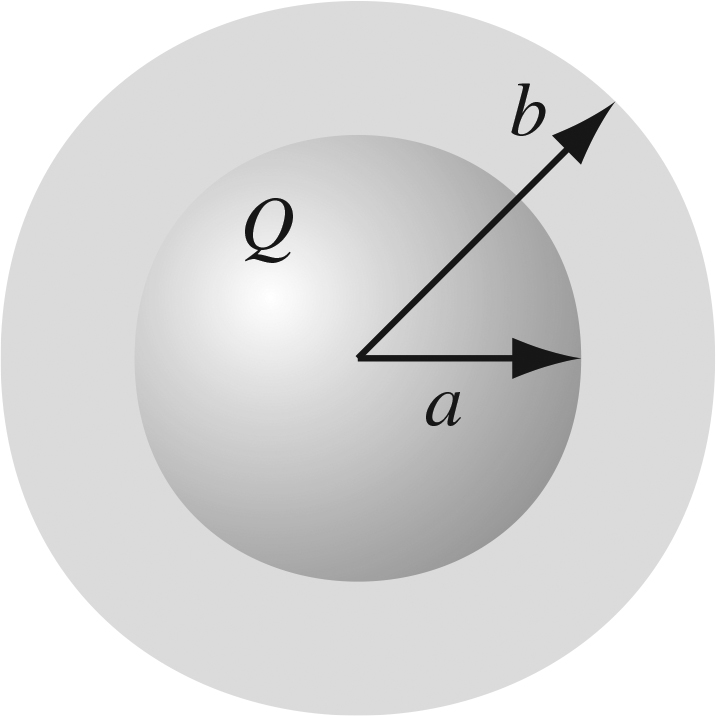
\includegraphics[width=3cm]{4_20.jpg} \hspace{2cm}
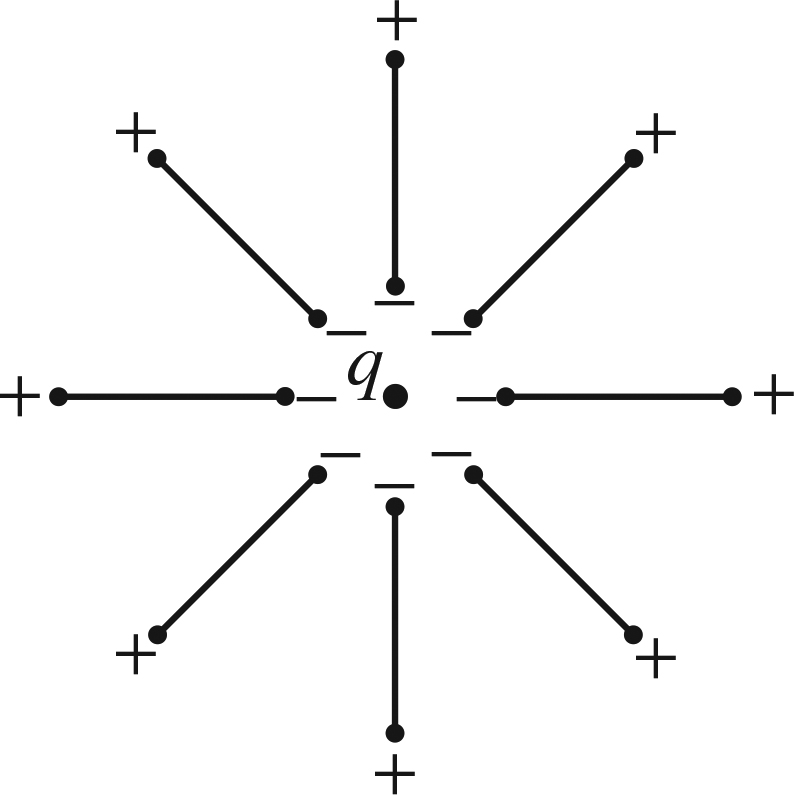
\includegraphics[width=3cm]{4_22.jpg}
\caption{\label{fig:shield} (Left) A metal sphere of charge $Q$ and radius $a$ is surrounded by linear dielectric material of permittivity $\epsilon$ out to radius $b$.  (RIght) A point charge embedded in a homogeneous linear dielectric with permittivity $\epsilon$.}
\end{figure}
\end{enumerate}

\end{document}
